\chapter{Implementation}

\section{Architecture}

\begin{figure}[h]
\centering
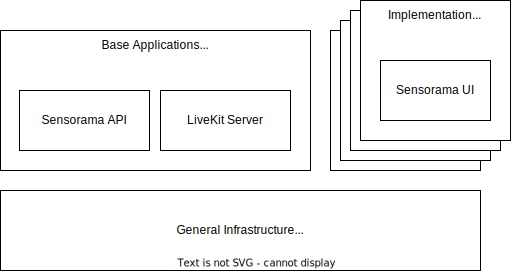
\includegraphics[scale=0.5]{04_Artefakte/01_Abbildungen/sensorama-stack}
\caption[Sensorama stack diagram]{The main components comprising the application architecture\protect}
\label{fig:sensoramaStack}
\end{figure}

The underlying hardware infrastructure is a bare-metal system running on-premises at the university. Due to the containerised packaging and deployment, it could also easily be deployed in a cloud environment or other hosting platform. No special hardware is required, and the system can run in any environment that provides network access, storage space and standard computing resources.

In an otherwise containerised application environment, the underlying software infrastructure is minimal. The components required are a Linux \ac{OS}, in this case, Ubuntu, with installations of Docker (with ContainerD) and Kubernetes.


\section{Application infrastructure}

While all the frameworks represented in \autoref{fig:mostUsedFrameworks} could be used to build an application as envisioned in this study, Vue is selected as the tool of choice due to the relatively high acceptance and the comparably easy learning curve. While it might not be the choice for large-scale or enterprise apps, the low entry barrier and the simple structure make it ideal to get an app up and running quickly, experiment with it and pass it on to others for hacking and custom modifications. To accelerate and simplify the initial development, the Quasar framework is used as it extends the basic functionality Vue provides by a \ac{UI} library with layout tools, preset interface elements and a comfortable development and deployment environment.

The choice for a backend framework lands on Feathers and, by extension, Koa. The simple structure and code generators allow for a speedy setup and deployment of a simple WebSockets \ac{API} that provides authentication and resource management. It is connected to a MongoDB database because there is no definitive initial plan of how the stored and retrieved resources are explicitly structured and typed. With a document store, the data can be easily overwritten with updated data and then wiped before the schema is fixed.

LiveKit is chosen as the WebRTC server implementation because it is effortless to set up as a container running along the Redis database in Kubernetes. It is extendable and scalable, and there is even a hosted variant for people who do not want to run their own server. While Mediasoup would allow a more precise implementation and probably more efficiency, the workload overhead for building everything already offered by LiveKit is too much effort for this kind of application. However, it might be interesting to see how components based on Mediasoup could be dropped into this application structure.

\section{Design paradigms}

The basic design paradigm used for the Sensorama application is that of an \ac{SPA}. As there is already a remote API involved in managing access to shared resources, the \ac{PWA} paradigm is not immediately of use. Still, it could be implemented with the existing application as well. It is an exclusively real-time application that uses WebSockets for all transmission between app components and uses the WebRTC standard for user communication. It is set up as a Monorepo, where all components are developed across languages in one repository.

\subsection{Application partitioning}

The application's custom part is partitioned into the user interface, which is a static built \ac{HTML}/\ac{CSS}/\ac{JS} bundle, the \ac{API}, which is a single-process Node.js application and the so-called \textquote{Data-Producers}, which are external native utilities written in Python and C++ that provide bridges to motion capture hardware.

\subsection{Coding style}

While the primarily favoured coding paradigm is object-oriented programming, this is only strictly applied to the core functionality. As some frameworks prefer different, more functional paradigms that are also compositional (Vue) or aspect-oriented (Feathers), it is beneficial not to enforce a singular coding style. This might be considered bad practice in a streamlined development environment, but it serves the purpose of a modular and somewhat unstable \textquote{single-use} application environment.

\subsection{Testing}

Only the core functionality deemed stable and reusable is unit-tested to provide a solid base functionality. The general user interface and data producers are considered transient because they serve a singular use case. These application components should be hackable and replaceable, so they are not tested in the scope of this study. However, more stable and general tools and extensions that warrant a unit testing setup could still be developed in the future.

\section{Application components}

The application comprises several third-party components merely deployed as-is (WebRTC, databases, static web server) and the custom-developed parts described here.

\subsection{Web frontend}

The web frontend provides the main entry point for the users. It allows authentication via a local username and password combination and then provides objects modelled as virtual \textquote{Spaces} that are the central anchor to organise all communications. A space object then maps to the the concept of a \textquote{chat room} in LiveKit or other real-time communications environments. Users can create spaces, name them and then join them, becoming active data producers, or choose to view them as passive spectators.

Depending on the participant's role, a space is rendered as a different set of components. Participants who actively join have access to a LocalProducer and a HeadTracker component. These components provide a direct link via WebSockets to the external data-producer utilities and a WebBluetooth connection to the custom head-tracking device built on Arduino. Those who only view the space do so via a dedicated scene viewer component that brings together all incoming streams and signals.

The frontend coordinates connections between the WebRTC server, the backend \ac{API} and the local utilities. It also implements the various web standard \ac{API}s needed for sound, graphics and communication.

\subsection{API backend}

In the backend, the \ac{API} server is only tasked with managing the basic connecting objects (spaces and users), general authentication, and generation of access tokens for the LiveKit server. Through its real-time implementation, it can notify connected clients of changes like other connecting users or updates to data. The Feathers framework exports its own client library that is specifically generated for the current server configuration and can be directly integrated into Vue by using a specific client adapter module (\textquote{feathers-pinia}) that handles authentication and basic \ac{CRUD} operations.

\subsection{Native utilities}

Three different native utilities are additionally implemented.

\subsubsection{General data producer}

This component is written as a \ac{CLI} utility in Python, as it implements various Python-specific extensions: the DepthAI framework, used to work with the Oak-D line of \ac{3D}-cameras, OpenVino for interacting with various \ac{ML} models for pose recognition or pointcloud extraction, Open3D for working with point-cloud data and general spatial operations and PyMotion, a library for working with recorded \ac{BVH} motion capture data files. Python also allows for easy statistical data analysis using NumPy, which is used for movement quality extraction.

\subsubsection{Captury data producer}

For real-time streaming of live motion capture data from the Captury Live system, there currently only exists a C++ client library provided by the system's manufacturer. Thus, this producer component has to be implemented separately and uses a C++-based WebSockets server streaming the library's received data.

\subsubsection{Head-tracker}

As there was no easily accessible and platform-independent head-tracking equipment, this component was quickly prototyped using a BluetoothLE-ready Arduino device (Nano RP2040 Connect) and an \ac{IMU} component for absolute orientation measurement by Adafruit (9-DOF Absolute Orientation IMU Fusion Breakout) that can be directly connected to the Arduino using the \ac{I2C} bus. The data read from the \ac{IMU} device is then posted as binary messages on a simple Bluetooth service. This device can be directly integrated using the browser's WebBluetooth web standard.
